\subsection{Deployment View}
The deployment view addresses the how and where of the \app system's execution, examining the distribution of components, the orchestration of services, and the overall infrastructure that supports the software. In other terms, this section is dedicated to a mapping between software artifacts that implement the logic that makes \app work and the hardware devices that are needed to concretely execute them.

This document aims to provide a comprehensive understanding of the architectural choices that facilitate efficient resource utilization, scalability to meet varying workloads, and the ability to adapt to evolving operational requirements. 

As in the previous sections, this view of the system is provided through multiple diagrams that go deeper and deeper into the details of the deployment environment. These diagrams are not exclusive to one another, rather they should be seen as a hierarchical illustration of the same concept, from a more high-level approach, to a more detailed insight.



\subsubsection{High-level Deployment View}
\begin{minipage}{\linewidth}
This diagram shows the bare minimum set of components that are needed to illustrate the deployment view for the \app system.

\vspace{1cm}
\begin{center}
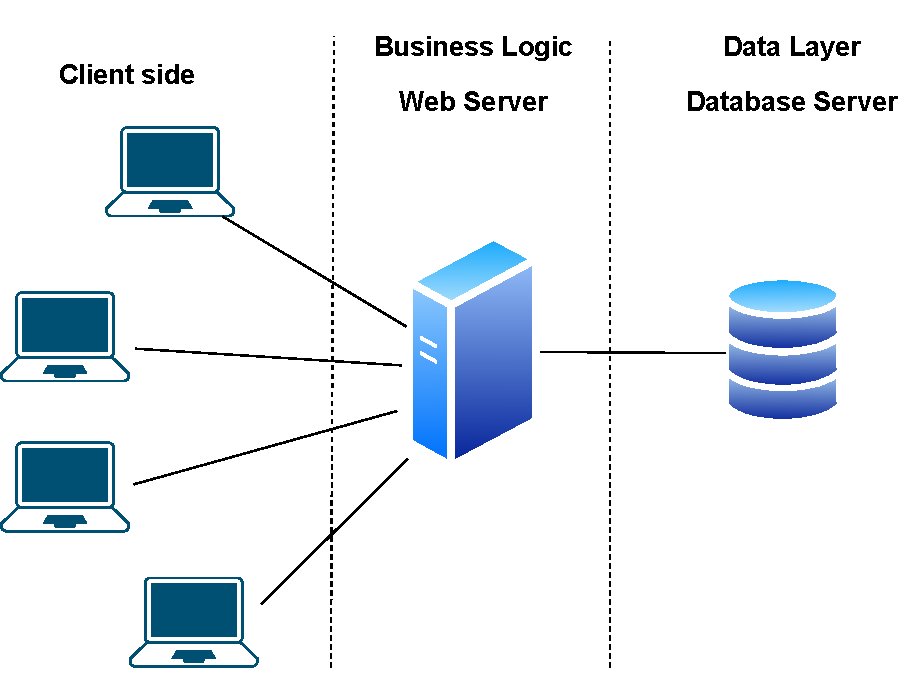
\includegraphics[width=0.7\linewidth]{1Deployment_High_Level}
\end{center}
\vspace{1.5cm}

\end{minipage}

As it is possible to see from the figure, from a deployment perspective, the \app platform can be classified as a three-tier architecture. The three distinct areas in the illustration represent the three tiers (layers) of the architecture, more specifically the client users (on the left), the server (in the center) and the data layer (on the right).

All users are equipped with a device with internet connection that is able to send and receive requests to the server hosting \app. The entire \app is hosted on a single remote server, where all microservices are launched as separate programs, interacting with each other. The data layer can be implemented with a remote Database server that provides persistent data support to the whole system.

This deployment architecture is very convenient for a series of reasons. First off, it allows for a complete separation of concerns between the various layers, in particular between the business logic of the application (hosted on the server) and the data layer (in the DBMS). Moreover, it is an extensible architecture that can be further developed and enlarged in order to accommodate for a varying workload. For instance, the data layer can be replicated on multiple servers, in order to increase performance for accessing and manipulating data. This same strategy can be adopted for the business layer in case of necessity.

\subsubsection{Detailed Deployment View}

\begin{minipage}{\linewidth}
	The following representation offers some more insights on how the software artifacts that implement the various components of the \app application map onto hardware elements.
	
	\vspace{2cm}
	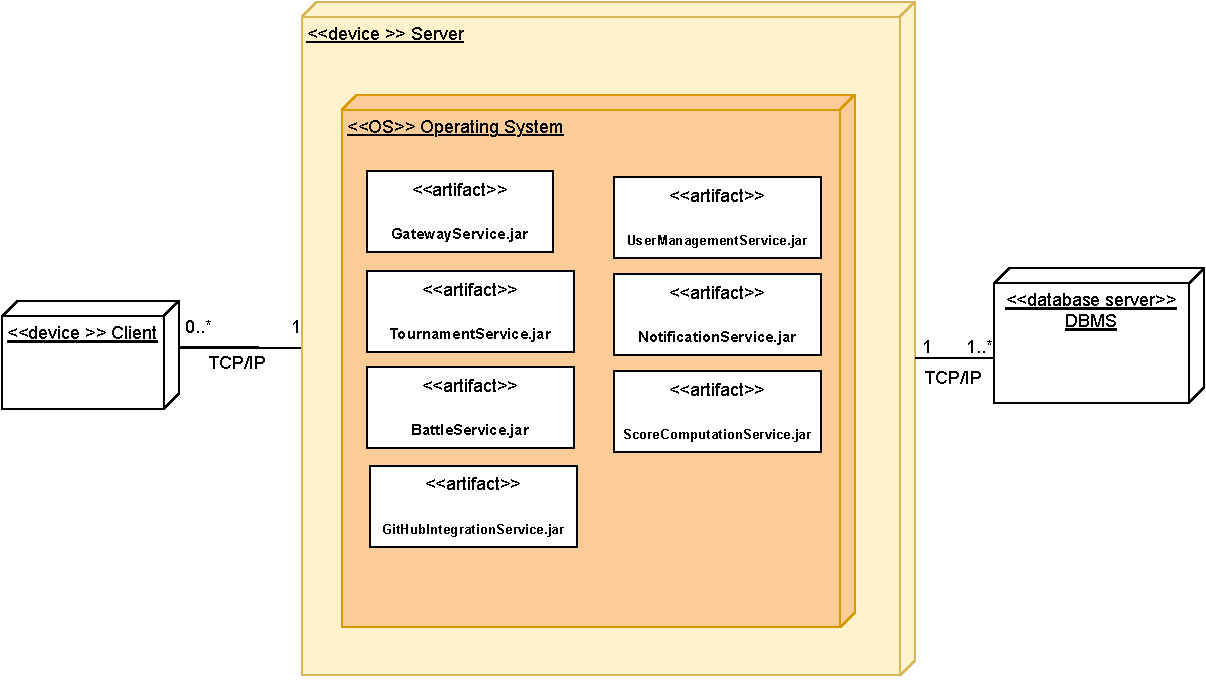
\includegraphics[width=\linewidth]{2DeploymentArtifacts}
	\vspace{1.5cm}
	
\end{minipage}

The major elements in the representation are still the same as in the previous description. On the left, the client side, equipped with a device that has internet access in order to communicate with the server over a TCP/IP protocol. The multiplicity specifications on the line that connects the client with the server shows that many clients can be interacting with the server simultaneously.

The server is the big box at the center of this diagram. The UML deployment diagram offers the possibility to show the execution environment of the \app system by nesting multiple boxes. 

All the microservices artifacts are mapped onto the single server instance. Indeed they are executed as separate processes inside the server machine.

Finally, on the right hand side, there is the data layer, which consists of a database server that is connected to the central server over the internet as well (TCP/IP protocol). 

This design has been chosen because it allows for smooth and easy extension of the system whenever it is needed. 
For instance, the DBMS can be replicated multiple times, in order to parallelise the requests coming from the server. 
If a more advanced distributed architecture was needed, the artifacts implementing the various microservices could simply be split across different nodes of the network and the overall system would still work correctly (with some settings and configurations).
The microservices themselves could be replicated inside the server machine in order to boost performance even more.
 

